% LuaLaTeX

\documentclass[a4paper, twoside, 12pt]{article}
\usepackage[latin]{babel}
%\usepackage[landscape, left=3cm, right=1.5cm, top=2cm, bottom=1cm]{geometry} % okraje stranky
\usepackage[landscape, a4paper, mag=1166, truedimen, left=2cm, right=1.5cm, top=1.6cm, bottom=0.95cm]{geometry} % okraje stranky

\usepackage{fontspec}
\setmainfont[FeatureFile={junicode.fea}, Ligatures={Common, TeX}, RawFeature=+fixi]{Junicode}
%\setmainfont{Junicode}

% shortcut for Junicode without ligatures (for the Czech texts)
\newfontfamily\nlfont[FeatureFile={junicode.fea}, Ligatures={Common, TeX}, RawFeature=+fixi]{Junicode}

% Hebrew font: http://scripts.sil.org/cms/scripts/page.php?site_id=nrsi&id=SILHebrUnic2
\newfontfamily\hebfont[Scale=1]{Ezra SIL}

\usepackage{multicol}
\usepackage{color}
\usepackage{lettrine}
\usepackage{fancyhdr}

% usual packages loading:
\usepackage{luatextra}
\usepackage{graphicx} % support the \includegraphics command and options
\usepackage{gregoriotex} % for gregorio score inclusion
\usepackage{gregoriosyms}
\usepackage{wrapfig} % figures wrapped by the text
\usepackage{parcolumns}
\usepackage[contents={},opacity=1,scale=1,color=black]{background}
\usepackage{tikzpagenodes}
\usepackage{calc}
\usepackage{longtable}
\usetikzlibrary{calc}

\setlength{\headheight}{14.5pt}

% Commands used to produce a typical "Conventus" booklet

\newenvironment{titulusOfficii}{\begin{center}}{\end{center}}
\newcommand{\dies}[1]{#1

}
\newcommand{\nomenFesti}[1]{\textbf{\Large #1}

}
\newcommand{\celebratio}[1]{#1

}

\newcommand{\hora}[1]{%
\vspace{0.5cm}{\large \textbf{#1}}

\fancyhead[LE]{\thepage\ / #1}
\fancyhead[RO]{#1 / \thepage}
\addcontentsline{toc}{subsection}{#1}
}

% larger unit than a hora
\newcommand{\divisio}[1]{%
\begin{center}
{\Large \textsc{#1}}
\end{center}
\fancyhead[CO,CE]{#1}
\addcontentsline{toc}{section}{#1}
}

% a part of a hora, larger than pars
\newcommand{\subhora}[1]{
\begin{center}
{\large \textit{#1}}
\end{center}
%\fancyhead[CO,CE]{#1}
\addcontentsline{toc}{subsubsection}{#1}
}

% rubricated inline text
\newcommand{\rubricatum}[1]{\textit{#1}}

% standalone rubric
\newcommand{\rubrica}[1]{\vspace{3mm}\rubricatum{#1}}

\newcommand{\notitia}[1]{\textcolor{red}{#1}}

\newcommand{\scriptura}[1]{\hfill \small\textit{#1}}

\newcommand{\translatioCantus}[1]{\vspace{1mm}%
{\noindent\footnotesize \nlfont{#1}}}

% pruznejsi varianta nasledujiciho - umoznuje nastavit sirku sloupce
% s prekladem
\newcommand{\psalmusEtTranslatioB}[3]{
  \vspace{0.5cm}
  \begin{parcolumns}[colwidths={2=#3}, nofirstindent=true]{2}
    \colchunk{
      \input{#1}
    }

    \colchunk{
      \vspace{-0.5cm}
      {\footnotesize \nlfont
        \input{#2}
      }
    }
  \end{parcolumns}
}

\newcommand{\psalmusEtTranslatio}[2]{
  \psalmusEtTranslatioB{#1}{#2}{8.5cm}
}


\newcommand{\canticumMagnificatEtTranslatio}[1]{
  \psalmusEtTranslatioB{#1}{temporalia/extra-adventum-vespers/magnificat-boh.tex}{12cm}
}
\newcommand{\canticumBenedictusEtTranslatio}[1]{
  \psalmusEtTranslatioB{#1}{temporalia/extra-adventum-laudes/benedictus-boh.tex}{10.5cm}
}

% volne misto nad antifonami, kam si zpevaci dokresli neumy
\newcommand{\hicSuntNeumae}{\vspace{0.5cm}}

% prepinani mista mezi notovymi osnovami: pro neumovane a neneumovane zpevy
\newcommand{\cantusCumNeumis}{
  \setgrefactor{17}
  \global\advance\grespaceabovelines by 5mm%
}
\newcommand{\cantusSineNeumas}{
  \setgrefactor{17}
  \global\advance\grespaceabovelines by -5mm%
}

% znaky k umisteni nad inicialu zpevu
\newcommand{\superInitialam}[1]{\gresetfirstlineaboveinitial{\small {\textbf{#1}}}{\small {\textbf{#1}}}}

% pars officii, i.e. "oratio", ...
\newcommand{\pars}[1]{\textbf{#1}}

\newenvironment{psalmus}{
  \setlength{\parindent}{0pt}
  \setlength{\parskip}{5pt}
}{
  \setlength{\parindent}{10pt}
  \setlength{\parskip}{10pt}
}

%%%% Prejmenovat na latinske:
\newcommand{\nadpisZalmu}[1]{
  \hspace{2cm}\textbf{#1}\vspace{2mm}%
  \nopagebreak%

}

% mode, score, translation
\newcommand{\antiphona}[3]{%
\hicSuntNeumae
\superInitialam{#1}
\includescore{#2}

#3
}
 % Often used macros
%%%% Preklady jednotlivych zpevu (nektere se opakuji, a je dobre mit je
% vsechny na jedne hromade)

\newcommand{\trOratioAnteOfficium}{\translatioCantus{Otevři, Pane, má ústa, abych chválil tvé svaté jméno.
Očisti mé srdce od všech marnivých, zvrácených a~jiných myšlenek, osvěť rozum, rozněť cit,
abych mohl důstojně, soustředěně a~zbožně recitovat a~vysloužil si být
vyslyšen před tváří tvé velebnosti. Skrze Krista…}}

\newcommand{\trOratioPostOfficium}{\translatioCantus{\textit{Následující modlitbu
opatřil pro ty, kdo ji zbožně vyřknou po hodinkách, zesnulý papež Lev X.
odpustky za hříchy vzniklé při konání hodinek z~lidské křehkosti. Říká se
vkleče.}
Svatosvaté a~nerozdílné Trojici, ukřižovanému lidství našeho Pána Ježíše
Krista, přeblažené a~přeslavné plodné neporušenosti vždy Panny Marie
i~souhrnu všech svatých buď ode všeho stvoření věčná chvála, čest a~sláva, nám
pak buď dáno odpuštění všech hříchů, po nekonečné věky věků. Amen.}}

% HOURS ---

\newcommand{\trAntI}{\translatioCantus{Jasné narození slavné Panny Marie,
z pokolení (dosl. ze semene) Abrahámova, vzešlé z kmene Judova, z rodu Davidova.}}
\newcommand{\trAntII}{\translatioCantus{Dnes je Narození svaté Panny 
Marie, jejíž předrahý život osvěcuje všechny církve.}}

\newcommand{\trAntIII}{\translatioCantus{Maria, jež vzešla 
z královského rodu, září; myslí i duchem ji zbožně prosíme, aby 
nám pomáhala svými přímluvami.}}

\newcommand{\trAntIV}{\translatioCantus{Srdcem i duchem pějme Kristu 
k slávě o této svaté slavnosti vznešené Rodičky Boží Marie.}}

\newcommand{\trAntV}{\translatioCantus{Příjemně \notitia{?} 
oslavujme Narození blahoslavené Marie,
aby se ona za nás přimlouvala u Pána Ježíše Krista.}}

\newcommand{\trCapituli}{\translatioCantus{Před věky, na počátku mě stvořil, potrvám věčně. Ve svatém Stanu jsem před ním konala službu.}}

\newcommand{\trRespVesp}{\translatioCantus{Buď zdráva, Maria,
plná milosti: \grestar{} Pán s tebou. \Vbardot{} Požehnaná jsi mezi ženami,
a požehnaný plod života (ve smyslu lůna, břicha) tvého.}}

\newcommand{\trVersus}{\translatioCantus{\Vbardot{} Dnes je Narození svaté Panny Marie. \Rbardot{} Jejíž předrahý život osvěcuje všechny církve.}}

\newcommand{\trAntMagnificatI}{\translatioCantus{Konejme památku
veledůstojného narození slavné Panny Marie,
jíž se dostalo mateřské důstojnosti bez ztráty panenské cudnosti.}}

% Tento preklad je vice nez nejisty a ani alternativy, ktere jsem
% videl, me nepresvedcily...
\newcommand{\trAntBenedictus}{\translatioCantus{Slavnostně slavme 
dnešní narození Marie, vždy Panny a Rodičky Boží: v něm se objevuje
vysokost trůnu (totiž Marie, trůnu Božího Syna), aleluja.}}

\newcommand{\trAntMagnificatII}{\translatioCantus{Tvé narození,
Bohorodičko Panno, vyhlásilo radost celému světu:
z tebe totiž vzešlo Slunce spravedlnosti, Kristus, náš Bůh:
jenž zrušil kletbu a dal nám požehnání: přemohl smrt a dal nám život věčný.}}

\newcommand{\trOrationis}{\translatioCantus{Prosíme tě, Bože, 
uděl svým služebníkům dar nebeské milosti,
aby těm, jimž slehnutím blahoslavené Panny vyvstal počátek spásy, 
slavnost k poctě jejího narození přinesla
rozhojnění pokoje.
Skrze tvého Syna, našeho Pána Ježíše Krista, který s tebou žije a kraluje,
Bůh, v jednotě Ducha svatého po všechny věky věků.}}

\newcommand{\trFideliumAnimae}{\translatioCantus{\Vbardot{} Duše věrných ať pro
milosrdenství Boží odpočívají v~pokoji. \Rbardot{} Amen.}}

% Completorium

\newcommand{\trJubeDomne}{\translatioCantus{Rač, pane, požehnat.}}

\newcommand{\trComplBenedictio}{\translatioCantus{Pokojnou noc a~svatou smrt
nechť nám dopřeje všemohoucí Pán. \Rbardot{} Amen.}}

\newcommand{\trComplLectioBr}{\translatioCantus{Buďte střízliví, bděte.
Váš protivník Ďábel obchází jako lev řvoucí a~hledá, koho by pohltil.
Postavte se proti němu pevní ve víře.  Ale ty, Pane, smiluj se nad námi.
\Rbardot{} Bohu díky.}}

\newcommand{\trComplAntI}{\translatioCantus{Rač se smilovati nade mnou,
Hospodine, a vyslyš mou modlitbu.}}

\newcommand{\trComplCapituli}{\translatioCantus{Jsi přece, Hospodine,
uprostřed nás a~jmenujeme se po tobě.  Neopouštěj nás, Pane, náš Bože.}}

\newcommand{\trRespCompl}{\translatioCantus{Do tvých rukou, Pane, \grestar{}
poroučím svého ducha. \Vbardot{} Ty mne zachráníš, Pane, Bože věrný.}}

\newcommand{\trComplVersus}{\translatioCantus{\Vbardot{} Střez mne jako zřítelnici oka,
aleluja. \Rbardot{} Ve stínu svých křídel uschovej mne, aleluja.}}

\newcommand{\trAntSalvaNos}{\translatioCantus{Ochraňuj nás, Pane, když
bdíme, a~buď s~námi, když spíme, ať bdíme s~Kristem a~odpočíváme v~pokoji.}}

\newcommand{\trComplOrationis}{\translatioCantus{Zavítej, prosíme, Pane, sem
do našeho příbytku a~daleko od něj zažeň všechny úklady nepřítele. Ať tu
bydlí tví svatí andělé a~tvoje požehnání buď nad ním stále. Skrze…}}

\newcommand{\trSalveRegina}{\translatioCantus{Zdrávas Královno, matko
milosrdenství, živote, sladkosti a naděje naše, buď zdráva!
K tobě voláme, vyhnaní synové Evy,
k tobě vzdycháme, lkajíce a plačíce
v tomto slzavém údolí.
A proto, orodovnice naše,
obrať k nám své milosrdné oči
a Ježíše, požehnaný plod života svého,
nám po tomto putování ukaž,
ó milostivá, ó přívětivá,
ó přesladká, Panno Maria!}}

\newcommand{\trOraProNobis}{\translatioCantus{\Vbardot{} 
Oroduj za nás, svatá Boží Rodičko,
\Rbardot{} aby nám Kristus dal účast na svých zaslíbeních.}}

% Matutinum

\newcommand{\trMatInvitatorium}{\translatioCantus{}}

\newcommand{\trMatVeniteA}{\translatioCantus{Pojďte, chvalme s~radostí Pána,
s~jásotem slavme Boha, svou spásu; předstupme před tvář jeho s~díky, písně plesu pějme jemu.}}

\newcommand{\trMatVeniteB}{\translatioCantus{Neboť Bůh veliký jest Hospodin, a~král nade všecky bohy.
Jsouť v~jeho ruce všecky hlubiny země, temena hor jsou majetek jeho.}}

\newcommand{\trMatVeniteC}{\translatioCantus{Jehoť jest moře, neb on je učinil; i~souš
je dílo jeho rukou. Pojďme, klanějme se, padněme, klekněme před Pánem, svým
tvůrcem. Jeť on Pán, náš Bůh, a~my jsme lid, jejž on vodí a~ovce, jež pase.}}

\newcommand{\trMatVeniteD}{\translatioCantus{Kéž byste poslechli dnes hlasu jeho:
,,Nezatvrzujte svých srdcí jak v~Hádce, jak v~Pokušení na poušti, kde vaši otcové pokoušeli mne,
zkoušeli mne, ač vídali skutky mé.``}}

\newcommand{\trMatVeniteE}{\translatioCantus{Čtyřicet roků mrzel jsem se na to pokolení
a~řekl jsem: ,,Lid je to myslí stále bloudící``! Oni však nechtěli znáti mé cesty, takže jsem
přisáhl ve svém hněvu: ,,Nedojdou odpočinku mého!\mbox{}``}}

\newcommand{\trMatAntI}{\translatioCantus{}}

\newcommand{\trMatAntII}{\translatioCantus{}}

\newcommand{\trMatAntIII}{\translatioCantus{}}

\newcommand{\trMatVersusI}{\translatioCantus{}}

\newcommand{\trMatAbsolutioI}{\translatioCantus{Vyslyš Pane Ježíši Kriste
prosby svých služebníků \gredagger{} a~smiluj se nad námi, \grestar{} jenž
s~Otcem a~Duchem…}}

\newcommand{\trMatBenedictioI}{\translatioCantus{Rač, pane, požehnat.
Věčný Otec nám stále žehnej. \Rbardot{} Amen.}}

\newcommand{\trMatLecI}{\translatioCantus{Kéž by mě zulíbal polibky svých úst. 
Tvé milování je nad víno lahodnější;
vybraně voní tvé voňavky;
rozlévající se olej je tvé jméno,
proto tě dívky milují.
Strhni mě za sebou, poběžme!
Král mě uvedl do svých komnat;
budeš nám radostí a jásotem.
Víc než víno oslavíme tvé milování;
věru po právu jsi milován!
Snědá jsem, a přece krásná, jeruzalémské dcery,
jako stany kedarské,
jako šalmské závěsy.
}}

\newcommand{\trMatRespI}{\translatioCantus{}}

\newcommand{\trMatBenedictioII}{\translatioCantus{Rač, pane, požehnat.
Jednorozený Boží Syn nám žehnej \grestar{} a nám pomáhej. \Rbardot{} Amen.}}

\newcommand{\trMatLecII}{\translatioCantus{Nehleďte na mou osmahlou pleť:
to mě slunce ožehlo.
Synové mé matky se na mne rozzlobili,
poslali mě hlídat vinice.
A svou vinici, tu jsem nehlídala!
Pověz mi tedy, ty, jehož miluje mé srdce:
kam zavedeš své stádo pást,
kde ho necháš za poledne odpočívat?
Abych už nebloudila jako tulačka
poblíž stád druhů tvých.
Nevíš-li to, nejrásnější z žen,
jdi po stopách stáda
a kůzlata svá zaveď, ať se pasou
poblíž obydlí pastýřů.
Ke své klisně zapřažené do vozu faraonova
tebe, mé milá, přirovnávám.
Stále krásné jsou tvé líce s náušnicemi
i tvé hrdlo v náhrdelnících.}}

\newcommand{\trMatRespII}{\translatioCantus{}}

\newcommand{\trMatBenedictioIII}{\translatioCantus{Rač, pane, požehnat.
Milost Ducha Svatého ať osvítí nám smysly \grestar{} i srdce. \Rbardot{} Amen.}}

\newcommand{\trMatLecIII}{\translatioCantus{Zhotovíme ti zlaté náušnice
a kuličky ze stříbra.
Když král stoluje,
vydechuje můj nard svou vůni.
Můj milý je polštářek s myrhou,
jenž mi odpočívá mezi ňadry.
Můj milý je hrozen šáchoru
ve vinicích v Engadi.
Jak jsi krásná, milá moje,
jak jsi krásná!
Tvé oči jsou holubice.
Jak jsi krásný, můj milý,
jak líbezný!
Naše lože je samá zeleň.
Trámoví našeho domu je z cedru,
naše ostění z cypřiše.}}

\newcommand{\trMatRespIII}{\translatioCantus{}}

\newcommand{\trMatAntIV}{\translatioCantus{}}

\newcommand{\trMatAntV}{\translatioCantus{}}

\newcommand{\trMatAntVI}{\translatioCantus{}}

\newcommand{\trMatVersusII}{\translatioCantus{}}

\newcommand{\trMatAbsolutioII}{\translatioCantus{
Tvá milost a laskavost nechť nám pomáhá, jenž žiješ a vládneš s Otcem a Svatým Duchem na věky věků.}}

\newcommand{\trMatBenedictioIV}{\translatioCantus{Rač, pane, požehnat.
Bůh Otec všemohoucí, \grestar{} buď k nám milostivý a odpouštějící. \Rbardot{} Amen.}}

\newcommand{\trMatLecIV}{\translatioCantus{}}

\newcommand{\trMatRespIV}{\translatioCantus{}}

\newcommand{\trMatBenedictioV}{\translatioCantus{}}

\newcommand{\trMatLecV}{\translatioCantus{}}

\newcommand{\trMatRespV}{\translatioCantus{}}

\newcommand{\trMatBenedictioVI}{\translatioCantus{Rač, pane, požehnat.
Bůh rozněť v nás oheň své lásky. \Rbardot{} Amen.}}

\newcommand{\trMatLecVI}{\translatioCantus{}}

\newcommand{\trMatRespVI}{\translatioCantus{}}

\newcommand{\trMatAntVII}{\translatioCantus{}}

\newcommand{\trMatAntVIII}{\translatioCantus{}}

\newcommand{\trMatAntIX}{\translatioCantus{}}

\newcommand{\trMatVersusIII}{\translatioCantus{}}

\newcommand{\trMatAbsolutioIII}{\translatioCantus{Z okovů našich hříchů,
\grestar{} vysvoboď nás všemohoucí a milosrdný Pán. \Rbardot{} Amen.}}

\newcommand{\trMatBenedictioVII}{\translatioCantus{Rač, pane, požehnat.
Čtení evangelia nechť je nám \grestar{} spásou a ochranou. \Rbardot{} Amen.}}

\newcommand{\trMatLecVIIa}{\translatioCantus{
  Rodokmen Ježíše Krista, syna Davidova, syna Abrahámova:
  Abrahám zplodil Izáka,
  Izák zplodil Jakuba.}}

\newcommand{\trMatLecVIIb}{\translatioCantus{}}

\newcommand{\trMatRespVII}{\translatioCantus{}}

\newcommand{\trMatBenedictioVIII}{\translatioCantus{Rač, pane, požehnat.
\Rbardot{} Amen.}}

\newcommand{\trMatLecVIII}{\translatioCantus{}}

\newcommand{\trMatRespVIII}{\translatioCantus{}}

\newcommand{\trMatBenedictioIX}{\translatioCantus{Rač, pane, požehnat.
Do společnosti občanů nebes \grestar{} ať nás dovede král andělů.
\Rbardot{} Amen.}}

\newcommand{\trMatLecIX}{\translatioCantus{}}

% from the Czech Liturgia horarum
\newcommand{\trTeDeum}{\begin{translatioMulticol}{3}

Bože, tebe chválíme, 
tebe, Pane, velebíme.

Tebe, věčný Otče, 
oslavuje celá země.

Všichni andělé, 
cherubové i~serafové,

všechny mocné nebeské zástupy 
bez ustání volají:

Svatý, Svatý, Svatý, 
Pán, Bůh zástupů.

Plná jsou nebesa i~země 
tvé vznešené slávy.

Oslavuje tě 
sbor tvých apoštolů,

chválí tě 
velký počet proroků,

vydává o~tobě svědectví 
zástup mučedníků;

a~po celém světě 
vyznává tě tvá církev:

neskonale velebný, 
všemohoucí Otče,

úctyhodný Synu Boží, 
pravý a~jediný,

božský Utěšiteli, 
Duchu svatý.

Kriste, Králi slávy, 
tys od věků Syn Boha Otce;

abys člověka vykoupil, 
stal ses člověkem a~narodil ses z~Panny;

zlomil jsi osten smrti 
a~otevřel věřícím nebe;

sedíš po Otcově pravici 
a~máš účast na jeho slávě.

Věříme, že přijdeš soudit, 

a~proto tě prosíme:
přispěj na pomoc svým služebníkům, 
vždyť jsi je vykoupil svou předrahou krví;

dej, ať se radují s~tvými svatými 
ve věčné slávě.

Zachraň, Pane, svůj lid, žehnej svému dědictví, 
veď ho a~stále pozvedej.

Každý den tě budeme velebit 
a~chválit tvé jméno po všechny věky.

Pomáhej nám i~dnes, 
ať se nedostaneme do područí hříchu.

Smiluj se nad námi, Pane, 
smiluj se nad námi.

Ať spočine na nás tvé milosrdenství, 
jak doufáme v~tebe.

Pane, k~tobě se utíkáme, 
ať nejsme zahanbeni na věky. 
\end{translatioMulticol}}

\newcommand{\trMatEvangelium}{\translatioCantus{
  Rodokmen Ježíše Krista, syna Davidova, syna Abrahámova:
  Abrahám zplodil Izáka,
  Izák zplodil Jakuba,
  Jakub zplodil Judu a jeho bratry,
  Juda zplodil Farese a Zaru z Tamary,
  Fares zplodil Esroma,
  Esrom zplodil Arama,
  Aram zplodil Aminadaba,
  Aminadab zplodil Naasona,
  Naason zplodil Salmona,
  Salmon zplodil Boaze z Rahaby,
  Boaz zplodil Jobeda z Rut,
  Jobed zplodil Jessea,
  Jesse zplodil krále Davida.
  David zplodil Šalomouna z Uriášovy ženy,
  Šalomoun zplodil Roboama,
  Roboam zplodil Abiu,
  Abia zplodil Asu,
  Asa zplodil Josafata,
  Josafat zplodil Jorama,
  Joram zplodil Oziáše,
  Oziáš zplodil Joatama,
  Joatam zplodil Achaze,
  Achaz zplodil Ezechiáše,
  Ezechiáš zplodil Manasesa,
  Manases zplodil Amona,
  Amon zplodil Josiáše,
  Josiáš zplodil Jechoniáše a jeho bratry;
  tehdy došlo k odvlečení do Babylonu.
  Po odvlečení do Babylonu:
  Jechoniáš zplodil Salatiela,
  Salatiel zplodil Zorobabela,
  Zorobabel zplodil Abiuda,
  Abiud zplodil Eljakima,
  Eljakim zplodil Azora,
  Ator zplodil Sadoka,
  Sadok zplodil Achima,
  Achim zplodil Eliuda,
  Eliud zplodil Eleazara,
  Eleatar zplodil Matana,
  Matan zplodil Jakuba,
  Jakub zplodil Josefa, manžela Marie,
  z níž se narodil Ježíš, který se nazývá Kristus.}}

\newcommand{\trTeDecetLaus}{\translatioCantus{Tobě chvála, Tobě zpěvy, Tobě
sláva, Bohu Otci i~Synu i~Svatému Duchu, na věky věků. \Rbardot{} Amen.}}

% MASS ---

\newcommand{\trIntroitus}{\translatioCantus{Radujme se všichni
v Pánu, slavíce svátek ke cti Panny Marie: z něj se radují andělé
a spoluchválí Božího Syna. \textit{\color{red}Žl.} Má ústa vydala dobré slovo,
přednáším svá díla králi.}}

\newcommand{\trGraduale}{\translatioCantus{Požehnaná a ctihodná jsi,
Panno Maria: nedotčená (co do panenství) jsi byla shledána matkou
Spasitele. \Vbardot{} Panno Boží Rodičko, ten, jehož nepojme ani celý svět,
se uzavřel do tvých útrob, když se stal člověkem.}}

\newcommand{\trAlleluia}{\translatioCantus{Aleluja. \Vbardot{} Skvělá slavnost
slavné Panny Marie, z pokolení (dosl. ze semene) Abrahámova, vzešlé z kmene 
Judova, z rodu Davidova.}}

\newcommand{\trOffertorium}{\translatioCantus{Blažená jsi, Panno Maria,
tys nosila Stvořitele všeho; porodila jsi toho, který tě utvořil,
a na věky zůstáváš Pannou.}}

\newcommand{\trCommunio}{\translatioCantus{Budou mě blahoslavit
všechna pokolení, protože mi učinil veliké věci ten, který je mocný.}}

% LITTLE HOURS ---

\newcommand{\trVersusTertia}{\translatioCantus{\Vbardot{} \Rbardot{}}}

\newcommand{\trCapituliEtSic}{\translatioCantus{
Tak jsem se usadila na Sionu a v milovaném městě jsem nalezla odpočinek,
v Jeruzalémě vykonávám svou moc.
Zakořenila jsem u lidu plného slývy, na panství Páně, v jeho dědictví.}}

\newcommand{\trVersusSexta}{\translatioCantus{\Vbardot{} \Rbardot{}}}

\newcommand{\trCapituliInPlateis}{\translatioCantus{
Na planině jako skořicovník a akant jsem vydávala vůni, jako vybraná myrha
jsem voněla.}}

\newcommand{\trVersusNona}{\translatioCantus{\Vbardot{} \Rbardot{}}}
 % Czech translations of the proper texts
\newfontface\GreGall{gregall.ttf}
\newfontface\GreGallModern{SGModern.ttf}
\directlua{dofile('gregall.lua')}
\newcommand{\gregallcharno}[3]{{\directlua{
  tex.sprint(gregallparse_neumes("\luaescapestring{#1}", "\luaescapestring{#2}", \luaescapestring{#3}))
}}}
\def\gregallchar{%
  \begingroup %
    \catcode`\~=12{}%
    \fontsize{8}{8}%
    \color{red}%
    \dogregallchar%
}
\def\dogregallchar#1{
    \gregallcharno{#1}{gregall}{0.8}%
  \endgroup %
}
\def\gregallmodchar{%
  \begingroup %
    \catcode`\~=12{}%
    \fontsize{16}{16}%
    \color{red}%
    \dogregallmodchar%
}
\def\dogregallmodchar#1{
    \gregallcharno{#1}{gregallmod}{1.6}%
  \endgroup %
}


\newcommand{\annusEditionis}{2015}

\def\hebinitial#1{%
\leavevmode{\newbox\hebbox\setbox\hebbox\hbox{\hebfont{#1}\hskip 1mm}\kern -\wd\hebbox\hbox{\hebfont{#1}\hskip 1mm}}%
}

%%%% Vicekrat opakovane kousky

\newcommand{\anteOrationem}{
  \rubrica{Ante Orationem, cantatur a Superiore:}

  \pars{Supplicatio Litaniæ.}

  \includescore{temporalia/supplicatiolitaniae.gtex}

  \pars{Oratio Dominica.}

  \includescore{temporalia/oratiodominica.gtex}

  \rubrica{Deinde dicitur ab Hebdomadario:}

  \includescore{temporalia/dominusvobiscum-solemnis.gtex}

  \rubrica{In choro monialium loco Dominus vobiscum dicitur:}

  \includescore{temporalia/domineexaudi.gtex}
}

\newcommand{\tuAutem}{
  \vfill

  \includescore{temporalia/tuautem.gtex}
}

\setlength{\columnsep}{30pt} % prostor mezi sloupci

%%%%%%%%%%%%%%%%%%%%%%%%%%%%%%%%%%%%%%%%%%%%%%%%%%%%%%%%%%%%%%%%%%%%%%%%%%%%%%%%%%%%%%%%%%%%%%%%%%%%%%%%%%%%%
\begin{document}

% Here we set the space around the initial.
% Please report to http://home.gna.org/gregorio/gregoriotex/details for more details and options
\setspaceafterinitial{2.2mm}{1}
\setspacebeforeinitial{2.2mm}{1}

\grechangedim{interwordspacetext}{0.38 cm plus 0.15 cm minus 0.05 cm}{1}%

% Here we set the initial font. Change 38 if you want a bigger initial.
% Emit the initials in red.
\def\greinitialformat#1{%
{\color{red}\fontsize{38}{38}\selectfont #1}%
}

\pagestyle{empty}

%%%% Titulni stranka
\begin{titulusOfficii}
\nomenFesti{In Festo Pentecostes.}
\celebratio{Duplex 1. classis.} % puvodne "cum Octava." Oktavy byly ale zruseny
\end{titulusOfficii}

% graphic
\vspace{1.5cm}
\begin{center}
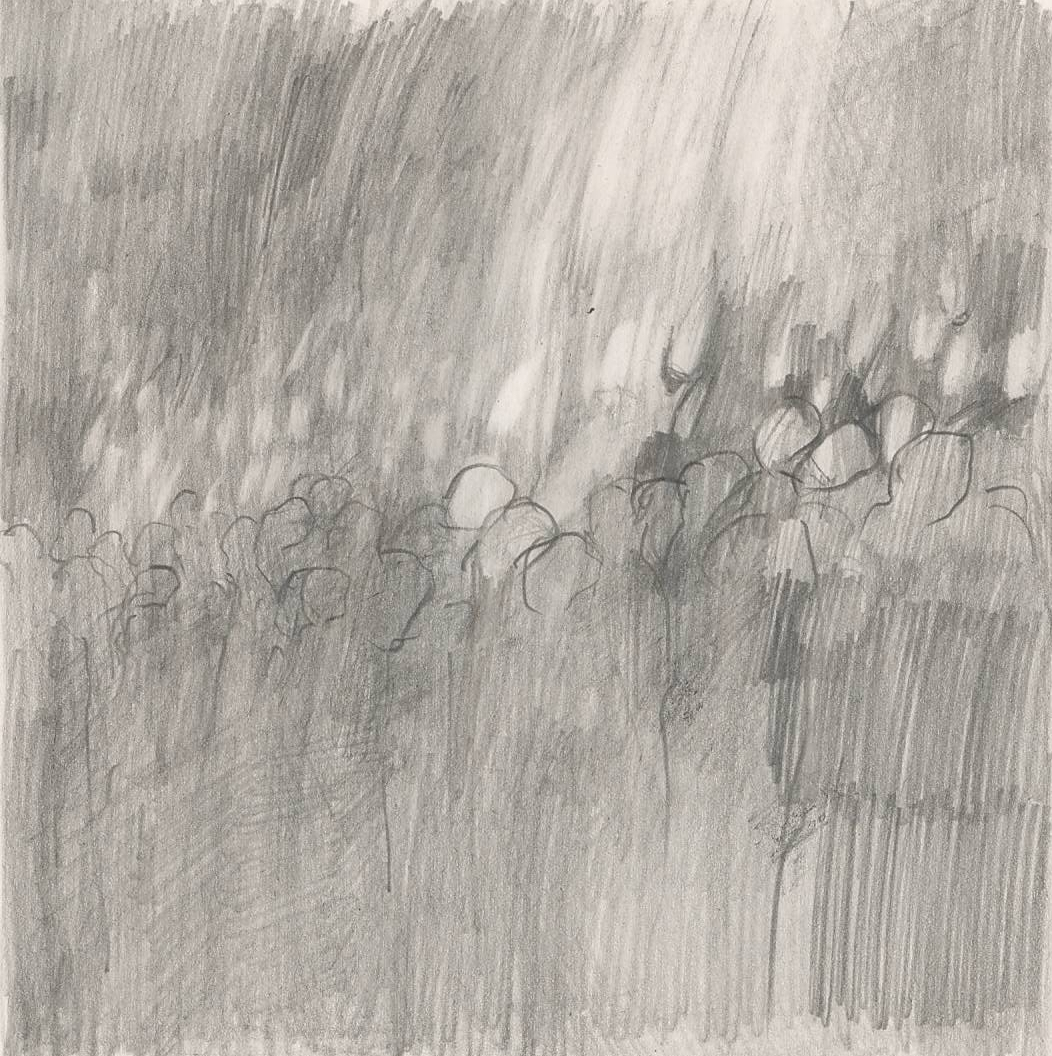
\includegraphics[width=8cm]{pentecostes.jpg}
\end{center}

\vfill

\begin{center}
Ad usum et secundum consuetudines chori \guillemotright{}Conventus Choralis\guillemotleft.

Editio Sancti Wolfgangi \annusEditionis
\end{center}

\pagebreak

\renewcommand{\headrulewidth}{0pt} % no horiz. rule at the header
\fancyhf{}
\pagestyle{fancy}

\pars{Léctio sancti Evangélii secúndum Ioánnem.} \scriptura{Io. 14, 23-31}

\textusEtTranslatio{
  Respóndit Iesus et dixit ei:
  Si quis díligit me, sermónem meum servábit, et Pater meus díliget eum,
  et ad eum veniémus, et mansiónem apud eum faciémus;
  Qui non díligit me, sermónes meos non servat.
  Et sermónem, quem audístis, non est meus:
  sed eius, qui misit me, Patris.
  Hæc locútus sum vobis apud vos manens.
  Paráclitus autem Spíritus Sanctus, quem mittet Pater in nómine meo,
  ille vos docébit ómnia, et súggeret vobis ómnia, quæcúmque díxero vobis.
  Pacem relínquo vobis, pacem meam do vobis:
  non quómodo mundus dat, ego do vobis.
  Non turbétur cor vestrum, neque formídet.
  Audístis quia ego dixi vobis: Vado et vénio ad vos.
  Si diligerétis me, gauderétis útique,
  quia vado ad Patrem: quia Pater maior me est.
  Et nunc dixi vobis, priúsquam fiat:
  ut, cum factum fúerit, credátis.
  Iam non multa loquar vobíscum:
  venit enim princeps mundi huius, et in me non habet quidquam.
  Sed ut cognóscat mundus quia díligo Patrem,
  et sicut mandátum dedit mihi Pater, sic fácio.
  Súrgite, eámus hinc.
}{\trMatEvangelium}{10cm}

\vfill
\pagebreak

\pars{Oratio ante divinum Officium.}

\lettrine{{\color{red}A}}{peri,} Dómine, os meum ad benedicéndum nomen sanctum tuum:
munda quoque cor meum ab ómnibus vanis, pervérsis, et aliénis
cogitatiónibus:
intelléctum illúmina, afféctum inflámma,
ut digne, atténte ac devóte hoc Offícium recitáre váleam,
et exaudíri mérear ante conspéctum Divínæ Maiestátis tuæ.
Per Christum, Dominum nostrum.
\Rbardot{} Amen.

Dómine, in unióne illíus divínæ intentiónis,
qua ipse in terris laudes Deo persolvísti,
has tibi Horas \rubricatum{(vel \textnormal{hanc tibi Horam})} persólvo.

\trOratioAnteOfficium

\vfill

\pars{Oratio post divinum Officium.}

\rubrica{
  Orationem sequentem devote post Officium recitantibus
  Leo Papa X. defectus, et culpas in eo persolvendo ex humana
  fragilitate contractas, indulsit, et dicitur flexis genibus.
}

\lettrine{{\color{red}S}}{acrosánctæ} et indivíduæ Trinitáti,
crucifíxi Dómini nostri Iesu Christi humanitáti,
beatíssimæ et gloriosíssimæ sempérque Vírginis Maríæ
fecúndæ integritáti, 
et ómnium Sanctórum universitáti
sit sempitérna laus, honor, virtus et glória
ab omni creatúra,
nobísque remíssio ómnium peccatórum,
per infiníta sǽcula sæculórum.
\Rbardot{} Amen.

\noindent \Vbardot{} Beáta víscera Maríæ Virginis, quæ portavérunt
ætérni Patris Fílium.\\
\Rbardot{} Et beáta úbera, quæ lactavérunt Christum Dominum.

\rubrica{Et dicitur secreto \textnormal{Pater noster.} et \textnormal{Ave María.}}

\trOratioPostOfficium

\vfill

\hora{In Vesperis.} %%%%%%%%%%%%%%%%%%%%%%%%%%%%%%%%%%%%%%%%%%%%%%%%%%%%%
\sideThumbs{Vesperæ}

\cantusSineNeumas

\includescore{temporalia/deusinadiutorium-solemnis.gtex}

\vfill
\pagebreak

\cantusCumNeumis

\pars{Psalmus 1.} \scriptura{Act. 2, 1; \textbf{H270}}

\antiphona{III a2}{temporalia/ant1.gtex}

\trAntI

\cantusSineNeumas

\scriptura{Ps. 109}

\includescore{temporalia/ps109-initium-iii-a2-auto.gtex}

\psalmusEtTranslatioT{temporalia/ps109-comb.tex}{10cm}

\vfill
\pagebreak

\pars{Psalmus 2.} \scriptura{Sap. 1, 7; \textbf{H270}}

\vspace{-4mm}

\antiphona{VIII G}{temporalia/ant2.gtex}

\trAntII

\scriptura{Ps. 110}

\includescore{temporalia/ps110-initium-viii-G-auto.gtex}

\psalmusEtTranslatioT{temporalia/ps110-comb.tex}{10cm}

\vfill
\pagebreak

\pars{Psalmus 3.} \scriptura{Act. 2, 4; \textbf{H270}}

\antiphona{VIII G}{temporalia/ant3.gtex}

\trAntIII

\scriptura{Ps. 111}

\includescore{temporalia/ps111-initium-viii-G-auto.gtex}

\psalmusEtTranslatioT{temporalia/ps111-comb.tex}{10cm}

\vfill
\pagebreak

\pars{Psalmus 4.} \scriptura{Dan. 3, 77.79; \textbf{H270}}

\antiphona{I a2}{temporalia/ant4.gtex}

\trAntIV

\scriptura{Ps. 112}

\includescore{temporalia/ps112-initium-i-a2-auto.gtex}

\psalmusEtTranslatioT{temporalia/ps112-comb.tex}{10cm}

\vfill
\pagebreak

\rubrica{In I. Vesperis:}

\pars{Psalmus 5.} \scriptura{\textbf{H271}}

\antiphona{VII c2}{temporalia/ant5.gtex}

\trAntV

\scriptura{Ps. 116}

\includescore{temporalia/ps116-initium-vii-c2-auto.gtex}

\psalmusEtTranslatioT{temporalia/ps116-comb.tex}{10cm}

\vfill
\pagebreak

\rubrica{In II. Vesperis:}

\pars{Psalmus 5.} \scriptura{\textbf{H271}}

\antiphona{VII c2}{temporalia/ant5.gtex}

\trAntV

\scriptura{Ps. 113}

\includescore{temporalia/ps113-initium-vii-c2-auto.gtex}

\psalmusEtTranslatioT{temporalia/ps113-comb.tex}{10cm}

\includescore{temporalia/ant5.gtex} % repeat the antiphon - new page

\vfill
\pagebreak

\raggedcolumns

% Capitulum. %%%
\cantusSineNeumas

\pars{Capitulum.} \scriptura{Act. 2, 1 - 2}

\includescore{temporalia/capitulum-CumComplerentur.gtex}

% preklad Jeruz. bible
\trCapituli

\vfill
\pars{Responsorium breve.}\rubrica{ - in I. vesperis:} \scriptura{\textbf{H269}}

\superInitialam{VI}
\includescore{temporalia/resp1v.gtex}

\trRespVespI

\vfill
\pagebreak

\pars{Responsorium breve.}\rubrica{ - in II. vesperis:}

\superInitialam{VI}
\includescore{temporalia/resp2v.gtex}

\trRespVespII

\vfill
\pagebreak

% Hymnus. %%%
\pars{Hymnus.}

\superInitialam{VIII}
\includescore{temporalia/hym-VeniCreator.gtex}
\begin{translatioMulticol}{4}
Duchu Tvůrce, přijď, navštiv nás,\\
přijď do srdce všech věrných svých\\
a~naplň je svou milostí,\\
vždyť ty sám jsi nás utvořil.\\
\\
Ty se nazýváš Těšitel,\\
Bůh nejvyšší nám tebe dal,\\
tys pramen živý, lásky žár,\\
pomazání jsi duchovní.\columnbreak

Dárce darů jsi sedmera,\\
prst pravice jsi Otcovy,\\
ty jsi ten Otcem slíbený,\\
správně dáváš nám promlouvat.\\
\\
V~duši světlo nám rozžehni\\
a~do srdce nám lásku vlej\\
a~naše tělo ubohé\\
stále silou svou posiluj.\columnbreak

Nepřítele pryč odežeň\\
a~ve světě svůj nastol mír,\\
nás cestou správnou vždycky veď,\\
ať nás mine vše škodlivé.\\
\\
Boha Otce nás nauč znát,\\
dej vyznávat nám Ježíše\\
a~tobě, Otci i~Synu\\
vírou se vždy víc otvírat.\columnbreak

Sláva Otci, i~Synu\\
zrozenému, který z~mrtvých\\
vstal, i~Utěšiteli,\\
na věky věků.\\
Amen.
\end{translatioMulticol}


\vfill
\pagebreak

\pars{Versus.}\rubrica{ - in I. vesperis:}

% Versus. %%%
\includescore{temporalia/versus-repleti.gtex}

\noindent \trVersusVespI

\vfill

\pars{Versus.}\rubrica{ - in II. vesperis:}

% Versus. %%%
\includescore{temporalia/versus-loquebantur.gtex}

\noindent \trVersusVespII

\vfill
\pagebreak

\cantusCumNeumis

\pars{Canticum B. Mariæ V.}\rubrica{ - in I. vesperis:} \scriptura{Io. 14, 18.28; ibid. 16, 22; \textbf{H267}}

\antiphona{I D*}{temporalia/ant-magn-vesp1.gtex}

\trAntMagnificatI

\vfill

\scriptura{Lc. 1, 46-55}

\cantusSineNeumas
\includescore{temporalia/magnificat-initium-i-D_.gtex}

\psalmusEtTranslatioT{temporalia/magnificat-comb.tex}{10cm}

%\includescore{temporalia/ant-magn-vesp1.gtex} % repeat the antiphon - new page

\vfill
\pagebreak

\pars{Canticum B. Mariæ V.}\rubrica{ - in II. vesperis:} \scriptura{\textbf{Sg. 388 p. 247}}

\cantusCumNeumis

\antiphona{I D*}{temporalia/ant-magn-vesp2.gtex}

\trAntMagnificatII

\vfill

\scriptura{Lc. 1, 46-55}

\cantusSineNeumas
\includescore{temporalia/magnificat-initium-i-D_.gtex}

% maly svindl, ale prizvukova struktura VIIIsoll-G2 a Isoll-D* je stejna
\psalmusEtTranslatioT{temporalia/magnificat-comb.tex}{10cm}

\includescore{temporalia/ant-magn-vesp2.gtex} % repeat the antiphon - new page

\vfill
\pagebreak

\anteOrationem

\pagebreak

% Oratio. %%%
\pars{Oratio.}

\includescore{temporalia/oratio.gtex}
\trOrationis

\vspace{1cm}
\rubrica{Hebdomadarius dicit iterum Dominus vobiscum. Postea cantatur a cantore:}
\vspace{2mm}

\rubrica{In I. Vesperis:}

\includescore{temporalia/benedicamus-solemnis-1vesp.gtex}

\rubrica{In II. Vesperis:}

\includescore{temporalia/benedicamus-solemnis-2vesp.gtex}

\vfill
\pagebreak

\hora{Ad Completorium.} %%%%%%%%%%%%%%%%%%%%%%%%%%%%%%%%%%%%%%%%%%%%%%%%%%%%%%%%%%
\sideThumbs{{\scriptsize{}Completorium}}

\rubrica{Lector petit benedictionem, dicens:}

\includescore{temporalia/jubedomnebenedicere.gtex}

\trJubeDomne

\vfill

\pars{Benedictio.}

\includescore{temporalia/benedictio-noctemquietam.gtex}

\trComplBenedictio

\vfill

\pars{Lectio brevis.} \scriptura{1Ptr. 5, 8-9}

\includescore{temporalia/lectiobrevis-fratressobrii.gtex}

\trComplLectioBr

\vfill

\noindent \Vbardot{} Adiutórium nostrum in nómine Dómini. \Rbardot{} Qui fecit cælum, et terram.

\vfill

\noindent Pater noster \rubricatum{quod dicitur totum secreto.}

\vfill
\pagebreak

\pars{Confessio.}

\noindent Confíteor Deo omnipoténti, beátæ Maríæ semper Vírgini, beáto
Michaéli Archángelo, beáto Ioánni Baptístæ, sanctis Apóstolis Petro
et Paulo, ómnibus Sanctis, et vobis fratres: quia peccávi nimis cogitatióne,
verbo et ópere: mea culpa, mea culpa, mea máxima culpa.
Ídeo precor beátam Maríam semper Vírginem, beátum Michaélum
Archángelum, beátum Ioánnem Baptístam, sanctos Apóstolos Petrum
et Paulum, omnes Sanctos, et vos fratres, oráre pro me ad Dóminum
Deum nostrum.

\vfill

\noindent \Vbardot{} Misereátur nostri omnípotens Deus, et, dimíssis peccátis nostris, perdúcat
nos ad vitam ætérnam. \Rbardot{} Amen.

\vfill

\noindent \Vbardot{} Indulgéntiam, absolutiónem et remissiónem peccatórum nostrórum tríbuat nobis
omnípotens et miséricors Dóminus. \Rbardot{} Amen.

\vfill

\rubrica{Et facta absolutione dicitur:}

\includescore{temporalia/convertenosdeus.gtex}

\vfill

\includescore{temporalia/deusinadiutorium-communis.gtex}

\vfill
\pagebreak

\pars{Psalmus 1.}

\antiphona{VIII G}{temporalia/ant-alleluia.gtex}

\scriptura{Ps. 4}

\includescore{temporalia/ps4-initium-viii-G-auto.gtex}

\psalmusEtTranslatioT{temporalia/ps4-comb.tex}{10cm}

\vfill
\pagebreak

\pars{Psalmus 2.} \scriptura{Ps. 90}

\psalmusEtTranslatioT{temporalia/ps90-comb.tex}{10cm}

\pagebreak

\pars{Psalmus 3.} \scriptura{Ps. 133}

\psalmusEtTranslatioT{temporalia/ps133-comb.tex}{10cm}

\vfill

\antiphona{VIII G}{temporalia/ant-alleluia.gtex}

\vfill

\pars{Hymnus.}

\antiphona{I}{temporalia/hym-TeLucis.gtex}
\begin{translatioMulticol}{3}
Než světlo zhasne prosíme\\
Tebe tvůrce všech pokorně,\\
abys nám ve své milosti\\
byl ochranou a~pomocí.\columnbreak

Ať vzdáleny jsou od nás sny\\
a~těžké noční přízraky.\\
Zdrť našeho nepřítele,\\
těla poskvrn ať ujdeme.\columnbreak

Tobě buď sláva, Ježíši,\\
národům že ses projevil,\\
Otci i~Duchu života\\
po věkoucí věky světa.\\
Amen.
\end{translatioMulticol}


\pagebreak

\pars{Capitulum.} \scriptura{Ier. 14, 9}

\includescore{temporalia/capitulum-tuautem.gtex}

% preklad Jeruz. bible
\trComplCapituli

\vfill

\pars{Responsorium breve.} \scriptura{Ps. 30, 6}

\superInitialam{VI}
\includescore{temporalia/resp-inmanus.gtex}

\trRespCompl
\vfill

\pars{Versus.} \scriptura{Ps. 16, 8}

\includescore{temporalia/versus-custodi.gtex}

\noindent \trComplVersus

\vfill
\pagebreak

\cantusCumNeumis

\pars{Canticum Simeonis.}

\antiphona{III a}{temporalia/ant-salvanos-antiquo.gtex}

\trAntSalvaNos

\scriptura{Lc. 2, 29-32}

\includescore{temporalia/nuncdimittis-initium-iii-a-auto.gtex}

\psalmusEtTranslatioT{temporalia/nuncdimittis-comb.tex}{10cm}

\vfill
\pagebreak

\pars{Oratio.}

\cantusSineNeumas

\includescore{temporalia/oratio-visita.gtex}

\trComplOrationis

\vfill

\includescore{temporalia/domineexaudi.gtex}

\vfill

\includescore{temporalia/benedicamus-minor.gtex}

\vfill

\pars{Benedictio.}

\noindent Benedícat et custódiat nos omnípotens et miséricors Dóminus, \gredagger{}
Pater, et Fílius, et Spíritus Sanctus. \Rbardot{} Amen.

\vfill
\pagebreak

\pars{Antiphona finalis B. M. V.}

\antiphona{V}{temporalia/an_regina_caeli_simplex.gtex}

\trReginaCaeli

\includescore{temporalia/versus-gaude.gtex}

\trGaudeEtLaetare

\vfill
\pagebreak

\hora{Ad Matutinum.} %%%%%%%%%%%%%%%%%%%%%%%%%%%%%%%%%%%%%%%%%%%%%%%%%%%%%%%%%%
\sideThumbs{Matutinum}

\vspace{2mm}

\includescore{temporalia/dominelabiamea.gtex}

\vspace{2mm}

\pars{Invitatorium.} \scriptura{Sap. 1, 7; Psalmus 94, 6; \textbf{H268}}

\vspace{-6mm}

\antiphona{V}{temporalia/matinv-AlleluiaSpiritus.gtex}

\trMatInvitatorium

\scriptura{Ps. 94. (Textus antiquus latinus); \textbf{H447}}

\vspace{-5mm}

\antiphona{V}{temporalia/venite5a.gtex}

\trMatVeniteA

\scriptura{Repetitur integrum Invitatorium.}

\includescore{temporalia/venite5b.gtex}

\trMatVeniteB

\scriptura{Repetitur altera pars Invitatorii.}

\rubrica{In sequenti Psalmi versu, ad verba \textnormal{veníte, adorémus et procidámus ante Deum}, genuflectitur.}

\includescore{temporalia/venite5c.gtex}

\trMatVeniteC

\scriptura{Repetitur integrum Invitatorium.}

\includescore{temporalia/venite5d.gtex}

\trMatVeniteD

\scriptura{Repetitur altera pars Invitatorii.}

\vfill
\pagebreak

\includescore{temporalia/venite5e.gtex}

\trMatVeniteE

\scriptura{Repetitur integrum Invitatorium.}

\includescore{temporalia/venite5f.gtex}

\scriptura{Repetitur altera pars Invitatorii. Denique repetitur integrum Invitatorium.}

\includescore{temporalia/matinv-AlleluiaSpiritus.gtex}

\vfill
\pagebreak

\pars{Hymnus.}

\vspace{-0.5cm}

\antiphona{VIII}{temporalia/hym-JamChristus.gtex}
{
\vspace{-0.5cm}
\setlength{\columnsep}{0pt} % prostor mezi sloupci
\begin{translatioMulticol}{5}
Již Kristus vstoupil ke hvězdám,\\
vrátil se, odkud vyšel sám,\\
aby dar Otcův zúročil\\
a Ducha Svatého dal nám.\\
\\
Den slavnosti pak přikvačil,\\
jenž divem sedminásobným\\
po zvratu světa sedmerém\\
svůj blažený čas vyznačil.\columnbreak

V hodinu třetí po ránu\\
znenáhla světem zahřmělo;\\
příchod Boha ta hodina\\
apoštolům zvěstovala.\\
\\
Z Otcova světla tu oheň je,\\
blažený je a přeslavný,\\
Kristovým věrným do srdce\\
žhnoucího tryská Slova žár.\columnbreak

Z plného srdce jásají\\
Duchem jsouce povzbuzeni\\
a hlasy znějí rozličné,\\
když Boží divy zvěstují.\\
\\
Řekům, Latincům, Barbarům,\\
všem jejich slova jasně zní,\\
protože k jejich údivu,\\
hovoří všemi jazyky.\columnbreak

Ale Židovstvo nevěrné\\
posedlé nevraživostí,\\
že prý moštem jsou opilí\\
střízlivým věrným vytýká.\\
\\
Když se div tento objevil,\\
vznešeně Petr promlouvá:\\
zlovolní pravdu nemají,\\
prorok Joel to dosvědčí.\columnbreak

Bohu Otci vždy sláva buď,\\
i Synu Zmrtvýchvstalému,\\
i Duchu Utěšiteli\\
po všechny věků okruhy.\\
Amen.
\end{translatioMulticol}

\setlength{\columnsep}{30pt} % prostor mezi sloupci
}

\vfill
\pagebreak

\pars{Psalmus 1.} \scriptura{Act. 2, 2; \textbf{H268}}

\antiphona{VIII c}{temporalia/matant1.gtex}

\trMatAntI

\scriptura{Ps. 47}

\includescore{temporalia/ps47-initium-viii-c-auto.gtex}

\psalmusEtTranslatioT{temporalia/ps47-comb.tex}{10cm}

\includescore{temporalia/matant1.gtex} % repeat the antiphon - new page

\vfill
\pagebreak

\pars{Psalmus 2.} \scriptura{Ps. 67, 29.30; \textbf{H268}}

\antiphona{VIII c}{temporalia/matant2.gtex}

\trMatAntII

\scriptura{Ps. 67}

\includescore{temporalia/ps67-initium-viii-c-auto.gtex}

\psalmusEtTranslatioT{temporalia/ps67-comb.tex}{10cm}

\includescore{temporalia/matant2.gtex} % repeat the antiphon - new page

\vfill
\pagebreak

\pars{Psalmus 3.} \scriptura{Ps. 103, 30; \textbf{H268}}

\vspace{-3mm}

\antiphona{VIII c}{temporalia/matant3.gtex}

\trMatAntIII

\scriptura{Ps. 103}

\includescore{temporalia/ps103-initium-viii-c-auto.gtex}

\psalmusEtTranslatioT{temporalia/ps103-comb.tex}{9.5cm}

\vfill
\pagebreak

\pars{Versus.} \scriptura{Sap. 1, 7}

\includescore{temporalia/versus-spiritus.gtex}

\noindent \trMatVersus

\vfill

\includescore{temporalia/oratiodominica-mat.gtex}

\vfill

\pars{Absolutio.}

\includescore{temporalia/absolutio-exaudi.gtex}

\trMatAbsolutioI

\vfill
\pagebreak

\includescore{temporalia/benedictio-solemn-evangelica.gtex}

\trMatBenedictioI

\vfill

\includescore{temporalia/tonus-lectionis-solemnis.gtex}

\vfill

% Léctio sancti Evangélii secúndum Ioánnem.
\pars{Lectio I.} \scriptura{Io. 14, 23-31}

\noindent Léctio sancti Evangélii secúndum \textit{Io}ánnem.

\textusEtTranslatio{
  In illo témpore: Dixit Iesus discípulis \textbf{su}is:~\gredagger{}
  Si quis díligit me, sermónem meum servábit, et Pater meus dí\textit{li}get eum,~\grestar{}
  et ad eum veniémus, et mansiónem apud eum fa\textit{ci}émus.
  \textit{Et} réliqua.
}{\trMatLecIa}{10cm}

% Homilía sancti Gregórii Papæ.
\scriptura{Homilia 30. in Evang.}

\noindent Homilía sancti Gregóri\textit{i} Papæ.

\textusEtTranslatio{
  Libet, fratres ca\textbf{rís}simi,~\gredagger{}
  evangelicæ verba lectiónis sub brevita\textit{te} transcúrrere,~\grestar{}
  ut post diutius liceat in contemplatióne tantæ solemnitátis im\textit{mo}rari.
  Hódie namque Spíritus Sanctus repentino sónitu super discípulos \textbf{ve}nit,~\gredagger{}
  mentesque carnalium in sui amórem \textit{per}mutávit,~\grestar{}
  et foris apparéntibus linguis \textbf{ig}neis,~\gredagger{}
  intus facta sunt cor\textit{da} flammántia;~\grestar{}
  quia dum Deum in ignis visióne suscepérunt, per amórem suáviter \textit{ar}sérunt.
  Ipse namque Spíritus \textit{San}ctus amor est:~\grestar{}
  unde et Ioánnes dicit Deus cá\textit{ri}tas est.
  Qui ergo mente integra De\textit{um} desíderat,~\grestar{}
  profecto iam habet, \textit{quem} amat.
  Neque enim quisquam posset De\textit{um} dilígere,~\grestar{}
  si eum quem díligit, non \textit{ha}béret.
}{\trMatLecIb}{10cm}

\tuAutem

\vfill
\pagebreak

\pars{Responsorium 1.} \scriptura{\Rbar{} Act. 2, 1.2 \Vbar{} ibidem; \textbf{H269}}

\responsorium{III}{temporalia/matresp1.gtex}{\trMatRespI}

\vfill
\pagebreak

\includescore{temporalia/benedictio-solemn-divinum.gtex}

\trMatBenedictioII

\vfill

\pars{Lectio II.} \scriptura{Homilia 30. in Evang.}

\textusEtTranslatio{
  Sed ecce, si unusquísque vestrum requirátur an di\textit{li}gat Deum:~\grestar{}
  tota fiducia et secura mente respon\textit{det,} Diligo.
  In ipso autem lectiónis exordio audístis quid Vé\textit{ri}tas dicit:~\grestar{}
  Si quis díligit me, sermónem meum \textit{ser}vábit.
  Probátio ergo di\textit{lec}tiónis,~\grestar{}
  exhibítio est \textit{o}peris.
  Hinc in epistola sua idem Ioánnes \textbf{di}cit:~\gredagger{}
  Qui dicit: Di\textit{li}go Deum,~\grestar{}
  et mandáta eius non custó\textit{dit,} mendax est.
  Vere étenim Deum dilígimus et mandáta eius \textit{cus}todímus,~\grestar{}
  si nos a nostris voluptátibus co\textit{ar}ctamus.
  Nam qui adhuc per illicita desidéria \textbf{dif}fluit,~\gredagger{}
  profecto De\textit{um} non amat:~\grestar{}
  quia ei in sua voluntáte con\textit{tra}dicit.
}{\trMatLecII}{10cm}

\tuAutem

\vfill
\pagebreak

\pars{Responsorium 2.} \scriptura{\Rbar{} Act. 2, 4.6 \Vbar{} ibid. 2, 4.11; \textbf{H269}}

\responsorium{II}{temporalia/matresp2.gtex}{\trMatRespII}

\vfill
\pagebreak

\includescore{temporalia/benedictio-solemn-adsocietatem.gtex}

\trMatBenedictioIII

\vfill

\pars{Lectio III.} \scriptura{Homilia 30. in Evang.}

\textusEtTranslatio{
  Et Pater meus diliget \textbf{e}um,~\gredagger{}
  et ad eum \textit{ve}niemus,~\grestar{}
  et mansiónem apud eum fa\textit{ci}émus.
  Pensate, fratres ca\textbf{rís}simi,~\gredagger{}
  quanta sit \textit{is}ta dígnitas,~\grestar{}
  habére in cordis hospítio advén\textit{tum} Dei.
  Certe, si domum nostram quisquam dives aut præpotens amícus in\textbf{tra}ret,~\gredagger{}
  omni festinántia domus tota \textit{mun}darétur,~\grestar{}
  ne quid fortásse esset, quod óculos amíci intrántis \textit{of}fenderet.
  Tergat ergo sordes pra\textit{vi} operis,~\grestar{}
  qui Deo præparat do\textit{mum} mentis.
  Sed vidéte quid Vé\textit{ri}tas dicat:~\grestar{}
  Veniemus, et mansiónem apud eum fa\textit{ci}émus.
  In quorúmdam étenim corda venit, et mansiónem non \textbf{fa}cit:~\gredagger{}
  quia, per compunctiónem quidem, Dei respec\textit{tum} percipiunt,~\grestar{}
  sed tentatiónis témpore hoc ipsum quo compúncti fúerant, oblivis\textbf{cún}tur;~\gredagger{}
  sicque ad perpetranda peccá\textit{ta} redeunt,~\grestar{}
  ac si hæc minime \textit{plan}xíssent.
}{\trMatLecIII}{10cm}

\tuAutem

\vfill
\pagebreak

% Te Deum

\pars{Hymnus Ambrosianus}

\superInitialam{III}
\includescore{temporalia/tedeum-solemnis.gtex}

\trTeDeum

\vfill
\pagebreak

% Evangelium

\includescore{temporalia/tonus-evangelii-b.gtex}

\vfill

\pars{Léctio san\textit{cti} Evangélii {\textnormal{\grestar{}}} secúndum Io\textit{án}nem.} \scriptura{Io. 14, 23-31}

\textusEtTranslatio{
  Respóndit Iesus \textit{et} dixit ei:~\grestar{}
  Si quis díligit me, sermónem meum servábit, et Pater me\textit{us} díliget eum,~\grestar{}
  et ad eum veniémus, et mansiónem apud e\textit{um} faciémus;~\grestar{}
  Qui non díligit me, sermónes meos non \textbf{ser}vat.
  Et sermónem, quem audís\textit{tis}, non est meus:~\grestar{}
  sed eius, qui misit me, \textbf{Pat}ris.
  Hæc locútus sum vobis apud vos \textbf{ma}nens.
  Paráclitus autem Spíritus Sanctus, quem mittet Pater \textit{in} nómine meo,~\grestar{}
  ille vos docébit ómnia, et súggeret vobis ómnia, quæcúmque díxero \textbf{vo}bis.
  Pacem relínquo vobis, pa\textit{cem} meam do vobis:~\grestar{}
  non quómodo mundus dat, ego do \textbf{vo}bis.
  Non turbétur cor vestrum, neque for\textbf{mí}det.
  Audístis quia ego dixi vobis: Vado et vénio \textbf{ad} vos.
  Si diligerétis me, gau\textit{de}rétis útique,~\grestar{}
  quia vado ad Patrem: quia Pater maior \textbf{me} est.
  Et nunc dixi vobis, \textit{pri}úsquam fiat:~\grestar{}
  ut, cum factum fúerit, cre\textbf{dá}tis.
  Iam non mul\textit{ta} loquar vobíscum:~\grestar{}
  venit enim princeps mundi huius, et in me non habet \textbf{quid}quam.
  Sed ut cognóscat mundus qui\textit{a} díligo Patrem,~\grestar{}
  et sicut mandátum dedit mihi Pater, sic \textbf{fá}cio.
  \textit{Súr}gite, e\textbf{á}mus hinc.
}{\trMatEvangelium}{10cm}

\vfill
\superInitialam{I}
\includescore{temporalia/tedecetlaus.gtex}

\trTeDecetLaus

\vfill
\pagebreak

\includescore{temporalia/domineexaudi.gtex}

\vfill

\pars{Oratio.}

\includescore{temporalia/oratio.gtex}
%\trOrationis

\vfill

\noindent \Vbardot{} Dómine, exáudi oratiónem meam.
\Rbardot{} Et clamor meus ad te véniat.

\vfill

% Nocturnale Romanum 2002, p. LXXVI Benedicamus Domino seems to match
% the one from Solemn Laudes.
\includescore{temporalia/benedicamus-solemnis-laud.gtex}

\vfill

\noindent \Vbardot{} Fidélium ánimæ per misericórdiam Dei requiéscant in pace.
\Rbardot{} Amen.

\trFideliumAnimae
\vfill
\pagebreak

\hora{Ad Laudes.} %%%%%%%%%%%%%%%%%%%%%%%%%%%%%%%%%%%%%%%%%%%%%%%%%%%%%%%%%%
\sideThumbs{Laudes}

% Psalmi festivi (AM33, pg. 721):
% 92, 99, 62, Dan3, 148+149+150

\vspace{1cm}
\includescore{temporalia/deusinadiutorium-communis.gtex}
\vspace{1cm}

\vfill
\pagebreak

\cantusSineNeumas

\pars{Psalmus 1.} \scriptura{Act. 2, 1; \textbf{H270}}

\antiphona{III a2}{temporalia/ant1.gtex}

\trAntI

\scriptura{Ps. 92}

\includescore{temporalia/ps92-initium-iii-a2-auto.gtex}

\psalmusEtTranslatioT{temporalia/ps92-comb.tex}{10cm}

\vfill
\pagebreak

\pars{Psalmus 2.} \scriptura{Sap. 1, 7; \textbf{H270}}

\antiphona{VIII G}{temporalia/ant2.gtex}

\trAntII

\scriptura{Ps. 99}

\includescore{temporalia/ps99-initium-viii-G-auto.gtex}

\psalmusEtTranslatioT{temporalia/ps99-comb.tex}{10cm}

\vfill
\pagebreak

\pars{Psalmus 3.} \scriptura{Act. 2, 4; \textbf{H270}}

\vspace{-4mm}

\antiphona{VIII G}{temporalia/ant3.gtex}

\trAntIII

\scriptura{Ps. 62}

\includescore{temporalia/ps62-initium-viii-G-auto.gtex}

\psalmusEtTranslatioT{temporalia/ps62-comb.tex}{10cm}

\vfill
\pagebreak

\pars{Psalmus 4.} \scriptura{Dan. 3, 77.79; \textbf{H270}}

\antiphona{I a2}{temporalia/ant4.gtex}

\trAntIV

\scriptura{Canticum trium puerorum, Dan. 3, 57-88 et 56}

\includescore{temporalia/dan3-initium-i-a2-auto.gtex}

\psalmusEtTranslatioT{temporalia/dan3-comb.tex}{10cm}

\rubrica{Hic non dicitur Gloria Patri, neque Amen.}
\vspace{1cm}

\hicSuntNeumae
\includescore{temporalia/ant4.gtex} % repeat the antiphon - new page

\vfill
\pagebreak

\pars{Psalmus 5.} \scriptura{\textbf{H271}}

\antiphona{VII c2}{temporalia/ant5.gtex}

\trAntV

%
\scriptura{Ps. 148.}

\includescore{temporalia/ps148-initium-vii-c2-auto.gtex}

\newlength{\psVItransW}
\setlength{\psVItransW}{10.5cm}

\psalmusEtTranslatioT{temporalia/ps148-comb.tex}{10cm}

\rubrica{Hic non dicitur Gloria Patri.}

%
\scriptura{Ps. 149.}

\includescore{temporalia/ps149-initium-vii-c2-auto.gtex}

\psalmusEtTranslatioT{temporalia/ps149-comb.tex}{10cm}

\rubrica{Hic non dicitur Gloria Patri.}

\vfill
\pagebreak

%
\scriptura{Ps. 150.}

\includescore{temporalia/ps150-initium-vii-c2-auto.gtex}

\psalmusEtTranslatioT{temporalia/ps150-comb.tex}{10cm}

\includescore{temporalia/ant5.gtex} % repeat the antiphon - new page

\vfill
\pagebreak

\cantusSineNeumas

\pars{Capitulum.} \scriptura{Act. 2, 1 - 2}

\includescore{temporalia/capitulum-CumComplerentur.gtex}

% preklad Jeruz. bible
\trCapituli

\vspace{1cm}
\pars{Responsorium breve.} \scriptura{Sap. 1, 7}

\superInitialam{VI}
\includescore{temporalia/respl.gtex}

\trRespLaudes
\vfill
\pagebreak

\pars{Hymnus.}

{
\grechangedim{interwordspacetext}{0.24 cm plus 0.15 cm minus 0.05 cm}{1}%
\superInitialam{I}
\includescore{temporalia/hym-BeataNobis.gtex}
\grechangedim{interwordspacetext}{0.38 cm plus 0.15 cm minus 0.05 cm}{1}%
}
\begin{translatioMulticol}{4}
Přinesl nám den radosti\\
roční běh času opět dnes,\\
když duch Pomocník září svou\\
kruh učedníků prostoupil.\\
\\
Za třepotání plamenů\\
uchvátil tvářnost jazyka,\\
aby z něj slova skanula,\\
jež láskou zapalovala.\columnbreak

Hovoří všemi jazyky,\\
strachem se chvějí zástupy,\\
soudíce, že jsou opilí,\\
kdo Duchem jsou naplněni.\\
\\
A to vše se přihodilo\\
když skončil čas velikonoc\\
ve svaté lhůtě, za kterou\\
káže vše Zákon odpustit.\columnbreak

Nyní Tě Bože přesvatý\\
s tváří skloněnou prosíme,\\
abys nám z nebes seslav je\\
tajemné dary ducha dal.\\
\\
Srdce kdysi posvěcené\\
naplnil jsi svou milostí,\\
odpusť nám naše přečiny\\
pokojný čas též dopřej nám.\columnbreak

Otci a Pánu sláva buď,\\
i Synu, který z mrtvých vstal,\\
i Duchu přímluv a pomoci\\
po všechny věků okruhy.\\
Amen.
\end{translatioMulticol}


\vfill
\pagebreak

\pars{Versus.}

% Versus. %%%
\includescore{temporalia/versus-repleti.gtex}

\noindent \trVersusLaudes

\vfill
\vspace{1cm}

\cantusCumNeumis

\pars{Canticum Zachariæ.} \scriptura{Io. 20, 22-23; \textbf{H271}}

\antiphona{VII a}{temporalia/ant-ben-laud.gtex}

\trAntBenedictus

\scriptura{Lc. 1, 68-79}

\includescore{temporalia/benedictus-initium-viisoll-a-auto.gtex}

\psalmusEtTranslatioT{temporalia/benedictus-comb.tex}{10cm}

\includescore{temporalia/ant-ben-laud.gtex} % repeat the antiphon - new page

\vfill
\pagebreak

\cantusSineNeumas

\anteOrationem

\pagebreak

% Oratio. %%%
\pars{Oratio.}

\includescore{temporalia/oratio.gtex}
\trOrationis

\vspace{1cm}
\rubrica{Hebdomadarius dicit iterum Dominus vobiscum. Postea cantatur a cantore:}
\vspace{2mm}

\includescore{temporalia/benedicamus-solemnis-laud.gtex}

\vfill
\pagebreak

\hora{Ad Tertiam.} %%%%%%%%%%%%%%%%%%%%%%%%%%%%%%%%%%%%%%%%%%%%%%%%%%%%%%%%%%
\sideThumbs{Tertia}

\vspace{1cm}
\includescore{temporalia/deusinadiutorium-communis.gtex}
\vfill
\pagebreak

\pars{Hymnus.}

\superInitialam{VIII}
\includescore{temporalia/hym-VeniCreator.gtex}
\begin{translatioMulticol}{4}
Duchu Tvůrce, přijď, navštiv nás,\\
přijď do srdce všech věrných svých\\
a~naplň je svou milostí,\\
vždyť ty sám jsi nás utvořil.\\
\\
Ty se nazýváš Těšitel,\\
Bůh nejvyšší nám tebe dal,\\
tys pramen živý, lásky žár,\\
pomazání jsi duchovní.\columnbreak

Dárce darů jsi sedmera,\\
prst pravice jsi Otcovy,\\
ty jsi ten Otcem slíbený,\\
správně dáváš nám promlouvat.\\
\\
V~duši světlo nám rozžehni\\
a~do srdce nám lásku vlej\\
a~naše tělo ubohé\\
stále silou svou posiluj.\columnbreak

Nepřítele pryč odežeň\\
a~ve světě svůj nastol mír,\\
nás cestou správnou vždycky veď,\\
ať nás mine vše škodlivé.\\
\\
Boha Otce nás nauč znát,\\
dej vyznávat nám Ježíše\\
a~tobě, Otci i~Synu\\
vírou se vždy víc otvírat.\columnbreak

Sláva Otci, i~Synu\\
zrozenému, který z~mrtvých\\
vstal, i~Utěšiteli,\\
na věky věků.\\
Amen.
\end{translatioMulticol}


\vfill
\pagebreak

\pars{Psalmus.} \scriptura{Sap. 1, 7; \textbf{H270}}

\antiphona{VIII G}{temporalia/ant2.gtex}

\trAntII

\scriptura{Ps. 118, 33-80}

\includescore{temporalia/ps118v_x-initium-viii-G-auto.gtex}

\psalmusEtTranslatioT{temporalia/ps118v_x-comb.tex}{10cm}

\includescore{temporalia/ant2.gtex} % repeat the antiphon - new page

\vfill
\pagebreak

\raggedcolumns

% Capitulum. %%%
\cantusSineNeumas

\pars{Capitulum.} \scriptura{Act. 2, 1 - 2}

\includescore{temporalia/capitulum-CumComplerentur.gtex}

% preklad Jeruz. bible
\trCapituli

\vfill

\pars{Versus.}

\includescore{temporalia/versus-spiritus-simplex.gtex}

\noindent \trMatVersus

\vfill

\rubrica{Ante Orationem, cantatur a Superiore:}

\pars{Supplicatio Litaniæ.}

\includescore{temporalia/supplicatiolitaniae.gtex}

\vfill

\pars{Oratio Dominica.}

\includescore{temporalia/oratiodominica-mat.gtex}

\vfill

\includescore{temporalia/domineexaudi.gtex}

\vfill
\pagebreak

% Oratio. %%%
\pars{Oratio.}

\includescore{temporalia/oratio.gtex}
\trOrationis

\vfill

\includescore{temporalia/benedicamus-minor.gtex}

\vfill

\noindent \Vbardot{} Fidélium ánimæ per misericórdiam Dei requiéscant in pace.
\Rbardot{} Amen.

\trFideliumAnimae

\vfill
\pagebreak

\hora{Ad Missam} %%%%%%%%%%%%%%%%%%%%%%%%%%%%%%%%%%%%%%%%%%%%%%%%%%%%%
\sideThumbs{Missa}

\pars{Antiphona ad introitum.} \scriptura{Sap. 1, 7; Psalmus 67; \textbf{E255}}

\cantusCumNeumis

\antiphona{VIII}{temporalia/introitus-SpiritusDomini.gtex}

\trIntroitus

\vfill

\pars{Kyrie VIII \textit{(De angelis)}.} \scriptura{XV. - XVI. s.}

\superInitialam{V}
\includescore{temporalia/viii-kyrie.gtex}

\vfill
\pagebreak

\pars{Gloria VIII.} \scriptura{XVI. s.}

\superInitialam{V}
\includescore{temporalia/viii-gloria.gtex}

\vfill
\pagebreak

\pars{Alleluia.} \scriptura{Ps. 103, 30; \textbf{C117}}

\antiphona{IV}{temporalia/alleluia-EmitteSpiritum.gtex}

\trAlleluiaEmitte

\vfill
\vspace{2cm}

\pars{Alleluia.} \scriptura{\textbf{Sg. 376 p. 296}}

\antiphona{II}{temporalia/alleluia-VeniSancte.gtex}

\trAlleluiaVeni

\vfill
\pagebreak

\pars{Sequentia.}

\antiphona{I}{temporalia/seq-VeniSancte.gtex}
{
\setlength{\columnsep}{5pt}
\begin{translatioMulticol}{5}
Přijď ó Duchu přesvatý,\\
rač paprsek bohatý\\
světla svého v nás vylít\\
\\
Přijdi, Otče nebohých,\\
dárce darů přemnohých,\\
rač nám mysli osvítit.\columnbreak

Božský Utěšiteli,\\
něžný duší příteli\\
rač nás mile zotavit.\\
\\
V práci libý pokoji,\\
smiřiteli v rozbroji\\
rač nás v pláči utišit.\columnbreak

Světlo duši blažící,\\
srdce v Tebe věřící\\
rač milostně naplnit.\\
\\
Člověk bez Tvé pomoci\\
slábne a je bez moci,\\
vše mu může uškodit.\columnbreak

Skvrny z našich duší smaž\\
a vyprahlá srdce svlaž,\\
raněné rač vyhojit.\\
\\
Srovnej co je zkřiveno,\\
zahřej co je studeno\\
a nedej nám zabloudit.\columnbreak

Rač nás v Tebe věřící,\\
vroucně Tebe prosící\\
dary sedmi podělit.\\
\\
Uděl v ctnosti prospěchu,\\
V smrti dodej útěchu\\
A dej v radost věčnou vjít.
\end{translatioMulticol}
}


\vfill
\pagebreak

\pars{Credo III.} \scriptura{XVII. s.}

{
\vspace{-0.22cm}
\vfill
\grechangedim{interwordspacetext}{0.28 cm plus 0.15 cm minus 0.05 cm}{1}%
\superInitialam{V}
\includescore{temporalia/credo-iii.gtex}
\grechangedim{interwordspacetext}{0.38 cm plus 0.15 cm minus 0.05 cm}{1}%
}

\vfill
\pagebreak

\pars{Offertorium.} \scriptura{Ps. 67, 29.30; \Vbardot{} ibid. 5.27.33.34; \textbf{E256}}

{
\grechangedim{interwordspacetext}{0.16 cm plus 0.15 cm minus 0.05 cm}{1}%
\antiphona{IV}{temporalia/offertorium-ConfirmaHoc.gtex}
\grechangedim{interwordspacetext}{0.38 cm plus 0.15 cm minus 0.05 cm}{1}%
}

\pagebreak

\trOffertorium

\vfill

\pars{Sanctus VIII.} \scriptura{(XI) XII. s.}

\superInitialam{VI}
\includescore{temporalia/viii-sanctus.gtex}

\vspace{1cm}
\pars{Agnus Dei VIII.} \scriptura{XV. s.}

\superInitialam{VI}
\includescore{temporalia/viii-agnusdei.gtex}

\vfill
\pagebreak

\pars{Communio.} \scriptura{Act. 2, 2.4.11; \textbf{E257}}

\vspace{-7mm}

\antiphona{VII}{temporalia/communio-FactusEst.gtex}

\trCommunio

\scriptura{Ps. 67, 2.4.5abc.5d.6.8.9.20.21.29.36}

\cantusSineNeumas
\includescore{temporalia/communio-versus-Exsurgat-initium.gtex}

\vspace{-5mm}

\psalmusEtTranslatioTS{temporalia/communio-versus-Exsurgat-comb.tex}{9.5cm}

\vfill
\pagebreak

\hora{Ad Sextam.} %%%%%%%%%%%%%%%%%%%%%%%%%%%%%%%%%%%%%%%%%%%%%%%%%%%%%%%%%%
\sideThumbs{Sexta}

\vspace{1cm}
\includescore{temporalia/deusinadiutorium-communis.gtex}
\vspace{1cm}

\pars{Hymnus.}

\antiphona{I}{temporalia/hym-RectorPotens.gtex}
\begin{translatioMulticol}{3}
Mocný vládce, pravý Bože\\
zlosti jež věcí mírníš všech,\\
září jitro jenž zaléváš\\
a žárem ohně poledne.\columnbreak

Uklidni plamen nesváru\\
rozhorlení nás ochraňuj.\\
Dopřej tělu zdravý klid\\
a mír pravý našim srdcím.\columnbreak

Sláva Otci, i Synu\\
zrozenému, který z mrtvých\\
vstal, i Utěšiteli,\\
na věky věků.\\
Amen.
\end{translatioMulticol}


\vfill
\pagebreak

\pars{Psalmus.} \scriptura{Act. 2, 4; \textbf{H270}}

\antiphona{VIII G}{temporalia/ant3.gtex}

\trAntIII

\scriptura{Ps. 118, 81-128}

\includescore{temporalia/ps118xi_xvi-initium-viii-G-auto.gtex}

\psalmusEtTranslatioT{temporalia/ps118xi_xvi-comb.tex}{10cm}

\includescore{temporalia/ant3.gtex} % repeat the antiphon - new page

\vfill
\pagebreak

\raggedcolumns

% Capitulum. %%%
\cantusSineNeumas

\pars{Capitulum.} \scriptura{Act. 2, 6}

\includescore{temporalia/capitulum-Facta.gtex}

% preklad Jeruz. bible
\trCapituliFacta

\vfill

\pars{Versus.}

\includescore{temporalia/versus-spiritusparaclitus.gtex}

\noindent \trVersusSexta

\vfill

\vfill

\rubrica{Ante Orationem, cantatur a Superiore:}

\pars{Supplicatio Litaniæ.}

\includescore{temporalia/supplicatiolitaniae.gtex}

\vfill

\pars{Oratio Dominica.}

\includescore{temporalia/oratiodominica-mat.gtex}

\vfill

\includescore{temporalia/domineexaudi.gtex}

\vfill
\pagebreak

% Oratio. %%%
\pars{Oratio.}

\includescore{temporalia/oratio.gtex}
\trOrationis

\vfill

\includescore{temporalia/benedicamus-minor.gtex}

\vfill

\noindent \Vbardot{} Fidélium ánimæ per misericórdiam Dei requiéscant in pace.
\Rbardot{} Amen.

\trFideliumAnimae

\vfill
\pagebreak

\hora{Ad Nonam.} %%%%%%%%%%%%%%%%%%%%%%%%%%%%%%%%%%%%%%%%%%%%%%%%%%%%%%%%%%
\sideThumbs{Nona}

\vspace{1cm}
\includescore{temporalia/deusinadiutorium-communis.gtex}
\vspace{1cm}

\pars{Hymnus.}

\antiphona{I}{temporalia/hym-RerumDeus.gtex}
\begin{translatioMulticol}{3}
Bože, jenž pro vše sílu máš\\
sám v sobě v nepohnutosti\\
a světlu dne různé po sobě\\
jdoucí doby jenž určuješ,\columnbreak

navečer dej nám jasnost zřít,\\
díky níž život nezhyne\\
a smrti svaté odměnu\\
navěky slavnou dostane.\columnbreak

Sláva tobě, Pane,\\
jenž ses z Panny narodil,\\
s Otcem i Svatým Duchem\\
na věčné věky.\\
Amen.
\end{translatioMulticol}


\vfill
\pagebreak

\pars{Psalmus.} \scriptura{\textbf{H271}}

\antiphona{VII c2}{temporalia/ant5.gtex}

\trAntV

\scriptura{Ps. 118, 129-176}

\includescore{temporalia/ps118xvii_xxii-initium-vii-c2-auto.gtex}

\psalmusEtTranslatioT{temporalia/ps118xvii_xxii-comb.tex}{10cm}

%\includescore{temporalia/ant5.gtex} % repeat the antiphon - new page

\pagebreak

\raggedcolumns

% Capitulum. %%%
\cantusSineNeumas

\pars{Capitulum.} \scriptura{Act. 2, 11}

\includescore{temporalia/capitulum-Judaei.gtex}

% preklad Jeruz. bible
\trCapituliJudaei

\vfill

\pars{Versus.}

\includescore{temporalia/versus-repleti-simplex.gtex}

\noindent \trVersusVespI

\vfill

\vfill

\rubrica{Ante Orationem, cantatur a Superiore:}

\pars{Supplicatio Litaniæ.}

\includescore{temporalia/supplicatiolitaniae.gtex}

\vfill

\pars{Oratio Dominica.}

\includescore{temporalia/oratiodominica-mat.gtex}

\vfill

\includescore{temporalia/domineexaudi.gtex}

\vfill
\pagebreak

% Oratio. %%%
\pars{Oratio.}

\includescore{temporalia/oratio.gtex}
\trOrationis

\vfill

\includescore{temporalia/benedicamus-minor.gtex}

\vfill

\noindent \Vbardot{} Fidélium ánimæ per misericórdiam Dei requiéscant in pace.
\Rbardot{} Amen.

\trFideliumAnimae

\vfill
\newpage
\RemoveSideThumbs
\pagestyle{empty}

%%% COLOPHON
\begin{center}
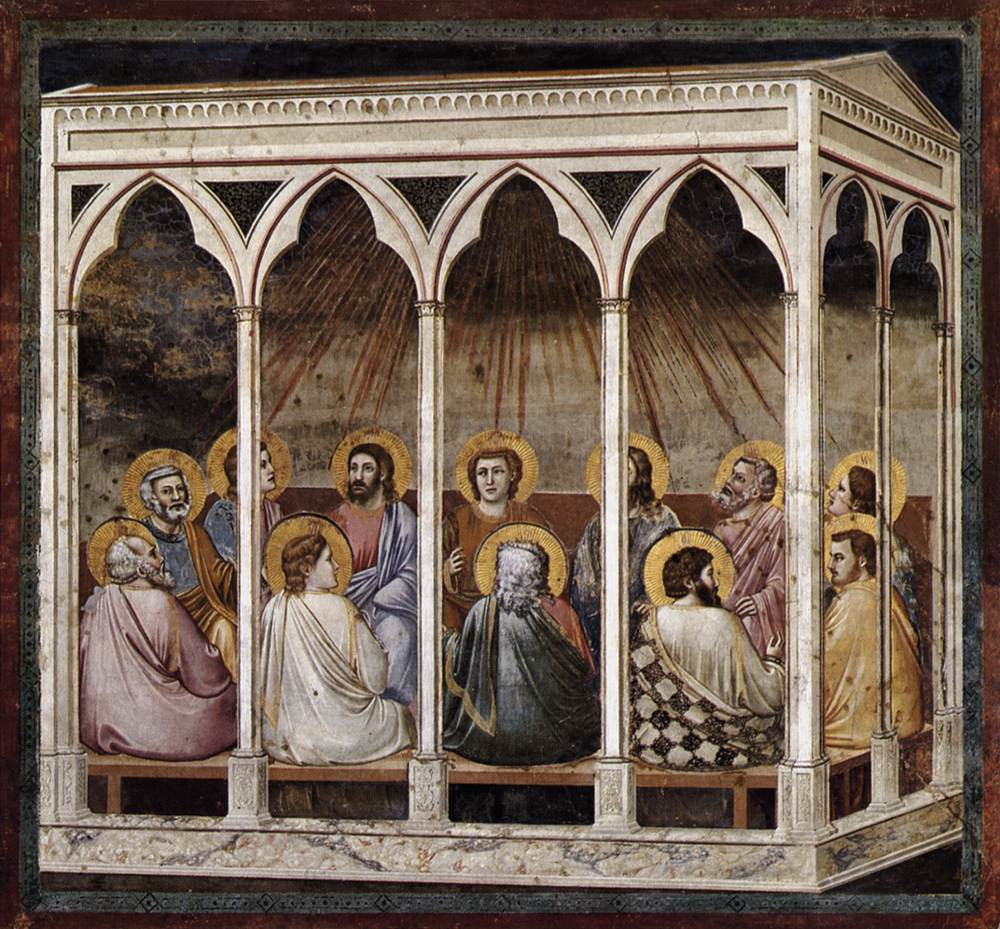
\includegraphics[width=6cm]{giotto.jpg}
\end{center}

\vfill

Fontes.
Textus et cantus officii divini secundum
Antiphonale Sacrosanctæ Romanæ Eclesiæ Pro Diurnis Horis, Romæ 1912
et Nocturnale Romanum, 2002, præter: psalmi 149 et 150 post
psalmum 148 in Laudibus additi secundum Antiphonale Monasticum pro Diurnis Horis,
Solesmis 1934; lectio sancti Evangelii et hymnus Te Decet Laus post hymnum
Ambrosianum additi secundum ritum monasticum vetum; responsorium breve
in Laudibus et Vesperis additum secundum Antiphonale Monasticum. /
Textus et cantus missæ secundum
Graduale triplex, Solesmis 1979. /
Translatio capituli et lectionis sumpta est ex:
Jeruzalémská bible, Praha-Kostelní Vydří 2009. /
Translationes psalmorum ex
Hejčl Jan: Žaltář čili Kniha žalmů, Praha 1922. /
Neumæ super canto missæ de codicibus Cantatorium, Stiftsbibl. 359 et Einsiedeln,
Stiftsbibl. 121 et neumæ super canto officii divini de codice Hartker,
Stiftsbibl. 391.

Collaborantes.
Textus latinos cantusque transcripsit et omnem laborem typographicum peregit
Jakub Jelínek et Jakub Pavlík. /
Psalmos in lingua bohemica de libro supra dicto transcripsit
Barbora Maturová et idem Jakub Jelínek. /
Václav Ondráček textus hymnorum, antiphonarum, homiliarum, benedictionum etc.
in linguam bohemicam transtulit. /
Filip Srovnal librum istum præparare mandavit et laborem exprobrationibus
utilissimis comitabatur. /
Štěpán Němec librum istum diligentissime examinavit, errores multos
inveniens. /
Terezie Regnerová imaginem titulum libri ornantem pinxit.

Instrumenta adhibita.
LuaTeX, %http://www.luatex.org /
Gregorio, %http://home.gna.org/gregorio /
typi Junicode. %http://junicode.sourceforge.net

\begin{center}
Liber hic imprimis ad usum chori
\guillemotright Conventus Choralis\guillemotleft\
paratus est
et secundum eius consuetudines.
http://www.introitus.cz

\vfill

{\large Editio Sancti Wolfgangi \annusEditionis.}

\vfill

Series \guillemotright Conventus\guillemotleft, vol. VII.

\vfill

http://stiwolfgangi.xf.cz

\end{center}

\vfill

\end{document}
